% Four-page letter version, written for IEEE Computer Architecture Letters (limit: 4 pages including figures, tables and references).
% Built here with article/twocolumn because IEEEtran.cls was not available offline; before submission move the body into the
% IEEE template (\documentclass[lettersize,journal]{IEEEtran}) via the IEEE Template Selector and re-check the page count.
\documentclass[10pt,twocolumn,a4paper]{article}
\usepackage[T1]{fontenc}
\usepackage[utf8]{inputenc}
\usepackage[top=1.7cm,bottom=1.8cm,left=1.55cm,right=1.55cm,columnsep=0.6cm]{geometry}
\usepackage{lmodern,booktabs,amsmath,graphicx}
\usepackage[expansion=false]{microtype}
\usepackage[hidelinks]{hyperref}
\newcommand{\UnitTests}{43}
\newcommand{\FuzzPrograms}{3000}
\newcommand{\FuzzDivergences}{0}
\newcommand{\FactNative}{107}
\newcommand{\FactLimb}{280}
\newcommand{\FactRatio}{2.62}
\newcommand{\SyscallCost}{275.1}
\newcommand{\YieldCost}{864.5}
\newcommand{\FrameBytes}{2064}
\newcommand{\TimerCost}{850.5}
\newcommand{\Quantum}{3000}
\newcommand{\Overhead}{22.1}
\newcommand{\KernelBytes}{19964}
\newcommand{\Opcodes}{59}

\setlength{\parskip}{0pt}\setlength{\parindent}{1em}
\renewcommand{\abstractname}{}
\makeatletter\renewcommand\section{\@startsection{section}{1}{\z@}{1.2ex plus .3ex}{0.6ex}{\normalfont\small\bfseries\scshape}}\makeatother
\title{\vspace{-1.2cm}\large\bfseries Amortizing MAC Checks in Tag-Free 128-Bit Capabilities:\\An Emulation Study\vspace{-0.3cm}}
\author{\small Durvesh M. Jadhav, independent researcher, ORCID 0009-0003-3779-2857\vspace{-0.4cm}}
\date{}
\begin{document}
\twocolumn[\maketitle\vspace{-0.9cm}
\begin{center}\begin{minipage}{0.93\textwidth}\small
\textbf{Abstract}---Capabilities that carry a keyed MAC in the pointer instead of an out-of-band tag need no tag memory, but appear to pay a MAC computation on every use. We study that cost on Veylith, an all-128-bit research ISA implemented twice (Python and C, cross-checked by differential fuzzing), whose \emph{Sigil} capability holds a 64-bit base, bounds, permissions and a 40-bit SipHash-based MAC in one 128-bit value. A per-register \emph{verified} bit, set when a capability is minted or first checked and cleared by any other write, lets the machine skip repeated checks without changing any architectural result. Over eighteen workloads, eleven compiler-generated, with footprints up to 512\,KiB, the bit removes every MAC check in array code that keeps a capability in a register (modelled slowdown 74--194\% without it at an 8-cycle MAC). In pointer-rich code it cannot: a binary search tree with capability links still needs a MAC for 49\% of uses, a modelled 126\% slowdown at $L{=}8$. A CHERI-style tag cache with 64 lines (4\,KiB of tag storage) costs under 0.6\% on every workload, but a 4-line cache thrashes on irregular code (up to 193\%), so on pointer-rich code a tagged design is likely faster unless the MAC latency is hidden. An unoptimised gate-level mapping of the MAC gives 269 gate levels, about 12--17 cycles. We state plainly that the latencies are parameters, the workloads small, and nothing here shows Sigil beating tagged capabilities.
\end{minipage}\end{center}\vspace{0.3cm}]

\section{Introduction}
Tagged capability machines such as CHERI \cite{cheri,cheriisa} keep a validity bit per capability-sized word in memory and a tag controller to serve it. Tag-free alternatives place a keyed MAC in the pointer: guarded pointers used a tag bit \cite{guarded}, while Intel's crypto-capabilities \cite{intelpat}, Cryptographic Capability Computing \cite{cthree} and cryptographically sealed pointers \cite{sealedptr} authenticate pointers cryptographically, within a 64-bit pointer that shortens the authenticator or the address. Authentication moves cost from memory to the core: every use seems to need a MAC. This letter measures that cost, and one way to avoid most of it, on a design where a 128-bit word leaves room for a 40-bit MAC beside a full 64-bit base. We do not claim the idea of tag-free authenticated capabilities, sealing or call gates is new; the contribution is the measurement and a reproducible platform.

\section{Design}
A Sigil is 128 bits: MAC[127:88], permissions[87:80], exponent[79:72], length multiplier[71:64], base[63:0]. It names $[\text{base},\text{base}+\ell 2^{e})$ with $1\le\ell\le256$. The MAC is the top 40 bits of SipHash-2-4 \cite{siphash} under a kernel-only key over bits[87:0]. Capability loads and stores trap on a bad MAC, a missing permission or an out-of-bounds offset, with immediate or register-indexed offsets. A forged value passes with probability $2^{-40}$; $300{,}000$ random forgeries were rejected. Capability-addressed memory is $2^{64}$ bytes, not the machine's $2^{128}$.

\emph{Verified bit.} Each register carries one microarchitectural bit. It is set when the machine itself mints the value (\texttt{cmint}, \texttt{cnarrow}, \texttt{cseal}, \texttt{cunseal}) or after a first successful MAC check of that register, and is cleared by every other write, by the register spill and refill of an isolated call, and by any key change. Memory remains tag-free, so a capability loaded from memory is unverified until first used. A differential test runs every random fuzz program with the bit on (with an audit that recomputes the MAC on every hit) and off and requires identical output, registers, memory and retired-instruction counts.

\section{Method}
All counts are retired instructions on a deterministic emulator, not cycles. Capability uses and MAC computations are measured, with and without the bit. Cost is modelled as $L$ extra cycles per MAC computation, shown for $L{=}2$ and $8$. The baseline is a CHERI-style tag cache (fully associative, LRU, 64-byte tag lines each covering 8\,KiB, 4 or 64 lines, 30-cycle miss) driven by the measured data-address stream. Eighteen workloads in three groups. Six hand-written (insertion sort, $8{\times}8$ matrix multiply, hash table, byte checksum, a linked list whose \texttt{next} field is itself a capability, and that list over 512\,KiB); six small programs from a toy Python-subset compiler (sieve, bubble sort, $6{\times}6$ matrix multiply, histogram, binary search, knapsack); and six larger benchmarks with footprints of 64--184\,KiB: merge sort, CSR sparse matrix-vector product, breadth-first search, longest-common-subsequence dynamic programming, a stencil sweep (all compiled), and a binary search tree whose child links are capabilities, built on the host and probed by 4096 lookups. Each runs through raw and capability code, and every result is checked against ordinary Python execution.

\section{Results}
\begin{table}[t]\centering\scriptsize\setlength{\tabcolsep}{2.5pt}
\begin{tabular}{@{}lrrrrrr@{}}\toprule
 & Cap.\ & MACs & \multicolumn{2}{c}{Slowdown \%, $L{=}8$} & \multicolumn{2}{c}{Tag cache \%}\\
Workload & uses & w/ bit & no bit & bit & 4 ln & 64 ln\\\midrule
\LetRows\bottomrule
\end{tabular}
\caption{Hand-written workloads. Slowdown is over the same capability code with free checks; tag cache uses a 30-cycle miss.}\label{t1}
\end{table}
\emph{Array code.} With one capability per array in a register, the bit leaves zero MAC computations after minting (Table~\ref{t1}); without it every access pays, a modelled 111--194\% at $L{=}8$. The six compiled programs behave the same: zero MACs with the bit, 74--171\% without. This is a result about register reuse, and it is a weak test: the toy compiler never spills a capability.

\begin{table}[t]\centering\scriptsize\setlength{\tabcolsep}{2pt}
\begin{tabular}{@{}lrrrr@{}}\toprule
Program & Cap.\ uses & MACs, bit & No bit, \% & Max regs\\\midrule
\LetCompRows\bottomrule
\end{tabular}
\caption{Compiler-generated programs (``No bit'': modelled slowdown at $L{=}8$ without the verified bit; ``Max regs'': most registers written in one 3000-instruction quantum). Every final variable and array equals ordinary Python execution of the same source.}\label{t2}
\end{table}
\emph{Pointers in memory.} When the \texttt{next} capability is loaded from memory, each hop is an unverified register: 5\,080 of 10\,240 uses need a MAC, and over 512\,KiB, 32\,766 of 65\,536. The modelled slowdown with the bit is 125\% and 64\% at $L{=}8$ (31\% and 16\% at $L{=}2$). Tag-free capabilities pay about one check per distinct pointer loaded; a tagged design does not pay it in cycles.

\begin{figure}[t]\centering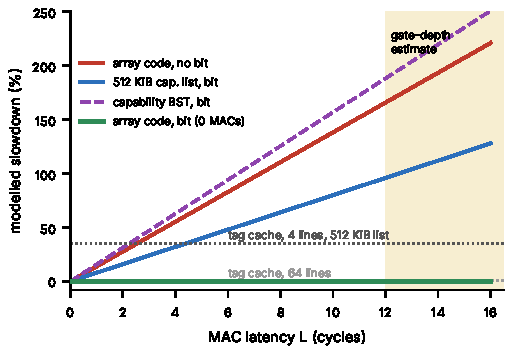
\includegraphics[width=0.97\columnwidth]{letter-fig.pdf}
\caption{Modelled slowdown against MAC latency $L$ (computed from the measured counts; the shaded band is the unoptimised gate-depth estimate of Section~\ref{sec:L}). Horizontal dotted lines are tag-cache costs for the 512\,KiB list at a 30-cycle miss, independent of $L$.}\label{f1}
\end{figure}
\begin{table}[t]\centering\scriptsize\setlength{\tabcolsep}{3.2pt}
\begin{tabular}{@{}lrrrrrrrr@{}}\toprule
 & Foot- & Cap.\ & MACs & \multicolumn{2}{c}{Slow.\ \%, $L{=}8$} & \multicolumn{3}{c}{Tag cache \% (lines)}\\
Benchmark & print KiB & uses & w/ bit & no bit & bit & 4 & 16 & 64\\\midrule
\MacroRows\bottomrule
\end{tabular}
\caption{Larger benchmarks. Tag-cache columns use a 30-cycle miss and 8\,KiB of data per 64-byte tag line.}\label{t3}
\end{table}
\emph{Larger benchmarks (Table~\ref{t3}).} The five compiled array benchmarks again need no MAC with the bit (112--180\% without it). The tree is the opposite case: each hop loads a capability from memory, 60\,210 of 122\,468 uses need a MAC, and the modelled slowdown is 126\% at $L{=}8$ even with the bit. Irregular access also stresses a tag cache: SpMV and BFS cost 122\% and 175\% with 4 tag lines (32\,KiB of data coverage), 0.2--0.9\% with 16 or 64; the tree needs 64 lines (0.3\%), and 16 lines still cost 29\%. A 64-line tag cache is only 4\,KiB, so on these benchmarks a modestly sized tag cache beats a 8-cycle MAC on pointer-rich code; the MAC design's case rests on simplicity, memory layout and compatibility, or on a MAC latency much below the gate-depth estimate.

\emph{Tag-cache baseline.} For the small workloads the tag cache has only compulsory misses (under 0.2\%). For the 512\,KiB walk a 4-line cache thrashes (35\%) while 64 lines, covering the footprint, cost 0.5\%. Which design wins therefore depends on $L$ and on the tag cache's size and miss penalty, neither of which this study measures.

\emph{Register state.} Instrumenting per 3000-instruction quantum, at most 16 of 128 registers were written in any quantum (13 in the compiled programs), so a hardware dirty mask would avoid roughly 87--96\% of register words moved on a context switch for programs like these.

\section{How large is $L$?}\label{sec:L}
We wrote the MAC in Verilog (eight SipRounds), checked it against the Python MAC on random vectors, and mapped it with Yosys to two-input gates. ABC does not run in the WebAssembly Yosys available, so nothing was optimised: one SipRound is 41 levels and 2\,136 gates; the unrolled MAC 269 levels and 17\,380 gates. At 16--24 levels per cycle that is 12--17 cycles unrolled and 16--24 iterative. A real flow would shorten this, SipHash-1-3 would remove three of eight rounds, but $L$ in the low teens is plausible, in which case the verified bit is a precondition of the design.

\section{Related work and positioning}
Guarded pointers \cite{guarded} are the closest ancestor (a pointer with a permission field and a power-of-two segment length, protected by a tag bit); CHERI \cite{cheri,cheriisa} keeps a tag per 128-bit word; the schemes of \cite{intelpat,cthree,sealedptr} authenticate pointers cryptographically inside a 64-bit pointer. The Sigil differs only in the design point a 128-bit word allows: a 64-bit base and a 40-bit MAC with nothing truncated or encrypted, on a machine whose registers, addresses and instructions are all 128 bits. A caching bit for verified pointers is a microarchitectural device analogous to caching a validated capability register; we have not found a published evaluation of it for MAC-authenticated capabilities, but our search was not exhaustive, so we do not claim it unprecedented.

\section{Limitations}
Emulation only: no timing, no process library, no area or energy. $L$ and the tag-cache miss penalty are parameters; the gate depth is not a timing result. The benchmarks are kernels of up to roughly $10^6$ instructions and at most 512\,KiB, hand-written or toy-compiled; the compiler has no functions and no spills; the tree is built on the host rather than by a capability-aware allocator; there is no real application, operating-system workload or multi-core behaviour. Two implementations by one author detect implementation slips, not specification errors. The 40-bit tag is a design choice, with no per-object revocation and no side-channel analysis. Nothing here shows Sigil is faster than tagged capabilities.

\section{Conclusion}
For tag-free MAC capabilities, caching verification per register is necessary: without it the modelled cost of array code is 74--194\% at an 8-cycle MAC, with it nearly zero. Pointer-chasing code over capabilities in memory still pays roughly one MAC per new pointer (126\% on a binary search tree at $L{=}8$), and the MAC's gate depth suggests this is expensive. A modest tag cache handles the same code at under 1\%, so the open problem for MAC capabilities is hiding verification latency (pipelined or speculative checks) and measuring it in a real flow. Code, data and scripts are in the public repository \texttt{sand-os-128} (\texttt{tools/cyclemodel.py}, \texttt{compiled\_study.py}, \texttt{macro\_bench.py}, \texttt{synth\_mac.py}, \texttt{rtl/sipmac.v}).

{\footnotesize\raggedright
\begin{thebibliography}{9}\setlength{\itemsep}{0pt}\setlength{\parsep}{0pt}
\bibitem{cheri} R.~N.~M. Watson et al., CHERI: A hybrid capability-system architecture for scalable software compartmentalization, \emph{IEEE S\&P}, 2015.
\bibitem{cheriisa} R.~N.~M. Watson et al., CHERI ISA (v9), Tech.\ Rep.\ UCAM-CL-TR-987, Univ.\ Cambridge.
\bibitem{guarded} N.~P. Carter, S.~W. Keckler, W.~J. Dally, Hardware support for fast capability-based addressing, \emph{ASPLOS}, 1994.
\bibitem{intelpat} Intel Corp., Crypto-enforced capabilities for isolation, US patent 10706164B2.
\bibitem{cthree} M.~LeMay et al., Cryptographic capability computing, \emph{MICRO}, 2021.
\bibitem{sealedptr} M.~Unterguggenberger, D.~Schrammel, L.~Lamster, P.~Nasahl, S.~Mangard, Cryptographically enforced memory safety, \emph{ACM CCS}, 2023.
\bibitem{siphash} J.-P. Aumasson, D.~J. Bernstein, SipHash: a fast short-input PRF, \emph{INDOCRYPT}, 2012.
\end{thebibliography}}
\end{document}
